\chapter{Números mágicos}
\label{c2}

O objetivo deste capítulo é apresentar

\section{Clusters}
\label{c2-clusters}

\textit{Clusters} são agregados de átomos ou moléculas, que variam desde dois à vários milhares de átomos e encontram-se na fronteira entre os átomos e o \textit{bulk}\footnote{\textit{Entende-se como "bulk" um conjunto de partículas sólidas grande o suficiente para que a média estatística de suas propriedades seja independente do número de partículas\cite{bulk}}}\cite{Heer,Brack}. 

No geral, os \textit{clusters} atômicos são classificados de acordo com seu tamanho: pequenos, médios ou grandes. Aglomerados classificados como pequenos, apresentam propriedades quânticas e possuem uma grande dependência com número de partículas que o compunha, essas propriedades não variam suavemente com seu tamanho, diferentemente dos \textit{clusters} médios e grandes. Normalmente os \textit{clusters} são ditos pequenos, quando contém mais do que algumas centenas ou quase mil partículas, os nano-agregados considerados grandes possuem muitas milhares de partículas e suas propriedades tendem a seguir a tendência das propriedades da matéria um \textit{bulk} \cite{livro_cluster}.

A análise da distribuição do tamanho dos \textit{clusters}, pode prover critérios fundamentais para o entendimento das tendências estruturais e energéticas dos mesmos. Buscando entender melhor as transições das propriedades dos \textit{clusters}, segundo Bernd v. Issendorff (2009), podemos começar os estudos pensando em uma descrição simples, porém suficiente, do modo como se comportam os elétrons de um metal. Assumindo um sistema de elétrons livres, isso implica que os elétrons da camada de valência se movem através de uma rede de metal infinita agindo como partículas livres. Assim, as funções de onda eletrônicas são apenas ondas planas tornando qualquer comprimento de onda possível. Uma mudança significativa ocorre quando o metal possuí dimensões nanoscópicas ou são nanopartículas. Agora, as funções de onda formam ondas estacionárias entre as superfícies da partícula, o que é possível somente para certos comprimentos de onda. Uma consequência direta é a discretização da densidade eletrônica de estados: a banda de valência contínua se divide em um número infinito de estados. Este é o chamado efeito de tamanho quântico, que pode levar a mudanças significativas propriedades das partículas de metal. Pode-se esperar que tais efeitos possam ser mais claramente vistos para um metal que se aproxime do comportamento ideal dos elétrons livres \cite{capitulo_livro_shell}. A Figura \ref{fig:transicao_cluster_solido} mostra a mudança das propriedades de um material enquanto \textit{clusters} e enquanto sólido, ilustrando o que foi dito.


\begin{figure}
  \centering
  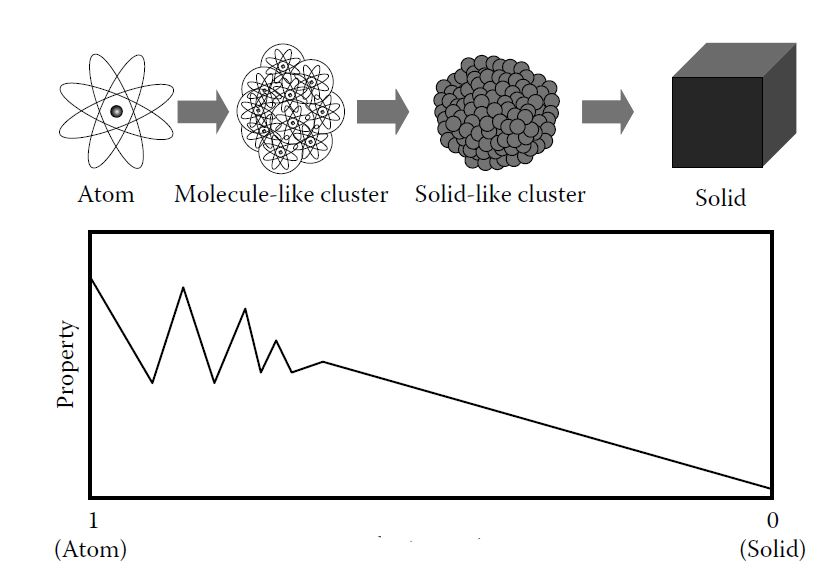
\includegraphics[width=0.8\textwidth]{images/clusters/atomo_cluste_solido}
  \caption{Esquema de transformação dimensional de átomos através de pequenos e grandes \textit{clusters} para o estado sólido. Quando os \textit{clusters} são pequenos cada átomo adicionado é importante, por isso as propriedades mudam
de forma abruptamente com o tamanho. Quando os \textit{clusters} se tornam grandes,
propriedades mudam suavemente\cite{cap06_Nanophysics}. Adaptado.  }
  \label{fig:transicao_cluster_solido}
\end{figure}

Uma das mudanças de propriedades interessantes é o surgimento de características semicondutoras em nanopartículas metálicas, que pode ser vista de Figura\ref{fig:carac_metal}. À medida que o número de átomos aumenta, também aumenta o número de níveis de energia disponíveis, até que a divisão entre níveis ocupados e desocupados se torna muito próxima e o \textit{cluster} começa a exibir comportamento metálico. Se aumentarmos um pouco o tamanho desta nanopartícula essas começaram a exibir comportamentos de pequenos pedaços do metal macroscópico. Abaixo desse tamanho crítico, os \textit{clusters} de elementos metálicos podem ter propriedades semelhantes a semicondutores.


\begin{figure}
  \centering
  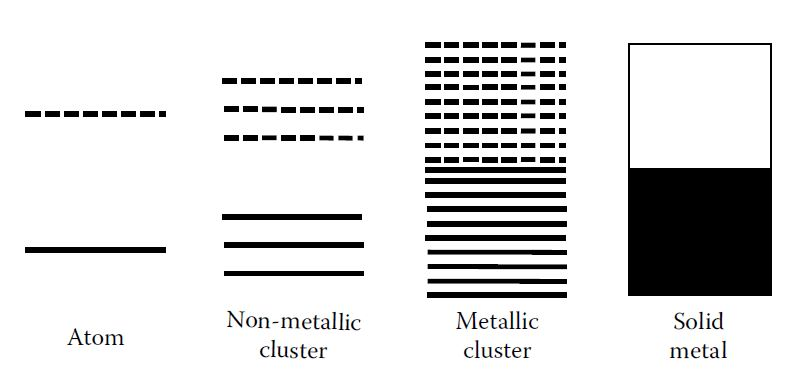
\includegraphics[width=0.7\textwidth]{images/clusters/carac_metal}
  \caption{ Esquema de transformação estrutural de energia a partir de átomos de metal através de pequenos e grandes \textit{clusters} para o metal sólido. Abaixo de um certo tamanho de \textit{clusters}, no qual as bandas vazia e povoada se fundem, um \textit{clusters} de átomos de metal pode ter uma estrutura de energia semelhante a um semicondutor.\cite{dissertacao_anderson}  }
  \label{fig:carac_metal}
\end{figure}



Deixando de lado os casos limites que geram ambiguidades, a diferença entre \textit{cluster} e moléculas encontra-se no fato que estas, no geral, possuem composições específicas e bem definidas e, na grande maioria dos casos, suas estruturas também são bem definidas, tendo  assim um número restrito de átomos; diferente um \textit{cluster}, como exemplo podemos citar um \textit{cluster} de prata que pode conter de 2, 15, 100, ou qualquer outro número de átomos de prata respeitando os limites impostos para que este ainda seja um \textit{cluster}. Esses por sua vez também não possuem uma estrutura única, como podemos ver na Figura \ref{fig:estrutura_cluster_ag}, e para sua maioria, à medida que o número de partículas do \textit{cluster} aumenta, o número de estruturas estáveis disponíveis torna-se mais abundante. 

\begin{figure}
  \centering
  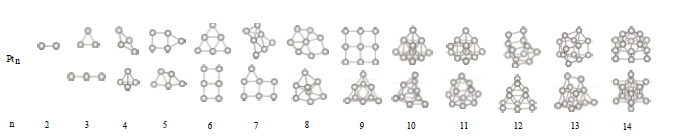
\includegraphics[width=1\textwidth]{images/clusters/estrutura_cluster_ag}
  \caption{ Exemplo de estruturas de \textit{clusters} de prata.\cite{dissertacao_anderson}  }
  \label{fig:estrutura_cluster_ag}
\end{figure}


O histórico de estudo da organização espacial dos arranjos atômicos frutificou em um Prêmio Nobel de Física em 1963. Metade do prêmio foi dado a Eugene Paul Wigner, por sua contribuição para a teoria do núcleo atômico e as partículas elementares,  e a outra metade foi partilhada por Maria Goeppert Mayer e J. Hans D. Jensen, pelas suas descobertas relativas à estrutura da casca nuclear. A análise das estruturas dos \textit{clusters} é fundamental para compreender suas propriedades e  dispor de seus potenciais tecnológicos, isso também torna-se muito importante para o domínio da estabilidade das nanopartículas. 



Em 1984, Knight et al \cite{electronic_Shell_sodium}, realizou um experimento com nanopartículas de sódio (Na), com N átomos por conglomerado (N = 4-100), e foram encontrado padrões, com picos bem definidos, no espectro de massa de \textit{clusters} de Na em fase gasosa, podendo ser visto na Figura \ref{fig:espec_na}(a). Cada pico do espectro representa o número de 
aglomerados de um determinado N detectado. Note a presença de picos maiores, quando comparado com os outros picos, para certas massas correspondentes à N = $8, 20, 40, 58$ e $92$, onde podemos notar padrões. Os \textit{clusters} mais abundantes
no espectro de massa são considerados relativamente mais estável. Podemos destacar a estrutura eletrônica dessas nanopartículas como a causa de maior estabilidade. Esses picos foram apelidados de \textit{clusters mágicos} ou \textit{clusters com números mágicos de átomos}.




\begin{figure}
  \centering
  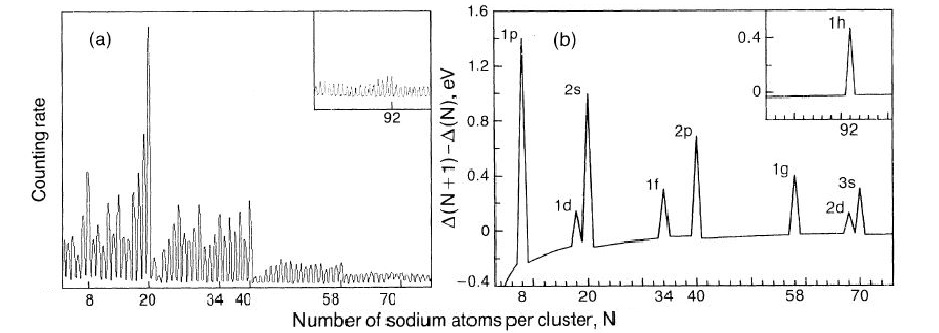
\includegraphics[width=1\textwidth]{images/clusters/NA_knight}
  \caption{(a) Espectro de massa de \textit{clusters} de sódio, N = 4-75.
  (b) A mudança calculada na diferença de energia eletrônica. Os picos protuberantes correspondem aos orbitais de casca fechada.\cite{electronic_Shell_sodium}  }
  \label{fig:espec_na}
\end{figure}


Podemos explicar a ocorrência desses \textit{clusters mágicos} foi suposto o efeitos de preenchimento de camadas eletrônicas, em que a combinação entre o espectro de estados
quantizados e o princípio de exclusão de Pauli resulta em efeitos de camada \cite{Brack}.O modelo quântico de \textit{Jellium} \cite{Heer}, foi usado com sucesso para explicar a ocorrência desses \textit{clusters mágicos} \cite{capitulo_livro_shell}.

As características dos espectros de massa de outros metais alcalinos e também dos metais nobres, seguem um padrão semelhante ao do sódio. Para as nanopartículas consideradas grandes, o padrão de números mágicos aparece diferente, e no geral ele é atribuído como uma consequência do preenchimento de camadas geométricas ou poliédricas de casca, assim o \textit{clusters} assume geometrias que minimizam a relação átomo-superfície uma vez que os átomos da superfície possuem um número menor de vizinhos do que os átomos internos, e o \textit{clusters} tende a preferir a estrutura de menor energia, maximizando a fração de átomo em massa. Essa estrutura geométrica da casca é bem conhecida nos \textit{clusters} de gás, e é característica de interações de curto alcance nas quais a tendência é para o empacotamento próximo do atomizado juntamente com a necessidade de minimizar a energia superficial \cite{capitulo_livro_shell}.




\section{Estrutura eletrônica \textit{shell model} para \textit{clusters} esféricos} \label{section_shell_model}

Pretendemos apresentar uma visão geral das características do sistema eletrônico \textit{shell model}.

O espectro de de massa da \ref{fig:espec_na} sugere que, os elétrons de valência nos \textit{clusters} de sódio são independentes e estão confinados em um potencial esfericamente simétrico. Assim como os átomos, as camadas eletrônicas de um \textit{cluster} com um número exato de elétrons para formar uma estrutura geometria poliédrica fechada, é muito estável. Assim que um átomo for adicionado a nanoestrutura, seu elétron de valência ocupará um estado com energia maior e assim a estabilidade do \textit{cluster} será reduzida, ocasionando uma rejeição deste estado e reduzindo sua sua abundância no espectro e isso explica a grade abundância após cada número de fechamento da casca.

Os números quânticos dos \textit{cluster} metálicos, são caracterizados de modo que cada casca é possuí um número quântico radial \textit{n} e o momento angular \textit{l}. Para um dado número quântico \textit{l}, o estado mais baixo tem $n = 1$, e assim por diante.


Uma abordagem com respaldo na mecânica quântica e que fornece uma descrição boa do comportamento observado na Figura \ref{fig:espec_na}, é considerarmos um elétron se movendo em um campo médio onde calculamos considerando que eles são partículas independentes movendo-se em um potencial parametrizado. O parâmetro básico do modelo é o raio de Wigner-Seitz, $r_{s}$, o raio de uma esfera contendo um elétron. O raio de um átomo de \textit{N} (ou elétron de valência) é dado por:

\begin{equation}
    R = r_{s}(N)^{\frac{1}{3}}
\end{equation}

É útil considerar a estrutura eletrônica surgindo com alguns potenciais simples. Para potenciais simétricos esfericamente, a função de onda é separável em uma parte radial e angular:

\begin{equation}
    \psi_{ n,l,m}(r, \theta, \phi) = R_{nl}(r)Y_{lm}(\theta, \phi)
\end{equation}

com os números quânticos familiares e $2(2l+1)$ de degenerescência (incluindo spin) em relação a \textit{m}. Três potenciais úteis para o estudo da física de \textit{cluster}, são os harmônicos, o poço quadrado e os potenciais Woods-Saxon mostrados na Figura \ref{fig:pocos}.

O potencial mais simples é o potencial do oscilador harmônico $V_{r}$:

\begin{equation}
    V(r)= \frac{1}{2}m\omega_0r^2
\end{equation}

o potencial do poço quadrado esférico (constante para $r<R$ e infinito para os demais). Como podemos ver na primeira coluna da Figura \ref{fig:pocos} os níveis de energia para o potencial do oscilador harmônico são igualmente espaçados, altamente degenerados e são rotulados pelo número quântico \textit{v}.

\begin{equation}
    E_{v}= \left(\frac{3}{2}+v\right)h\omega_0
\end{equation}


\begin{figure}
  \centering
  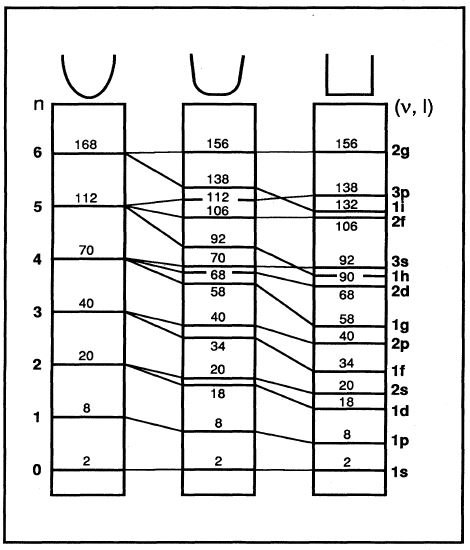
\includegraphics[width=0.5\textwidth]{images/clusters/pocos}
  \caption{(a) Espectro de massa de \textit{clusters} de sódio, N = 4-75.
  (b) A mudança calculada na diferença de energia eletrônica. Os picos protuberantes correspondem aos orbitais de casca fechada.\cite{electronic_Shell_sodium}  }
  \label{fig:pocos}
\end{figure}


